\documentclass[%
    %handout
]{beamer}
\usepackage{graphicx} % For including single page pdfs
\usepackage{bm}       % bold math
\usepackage{pgffor}   % for loop
\usepackage{tikz}
\usepackage{multimedia}
\usepackage{layouts}
\usepackage{hyperref}

% todo 
% sampling figure
% mcmc for ligo case
% trim talk
% mention bayesian vs frequentist


\newcommand{\lik}{\mathcal{L}}
\newcommand{\posterior}{\mathcal{P}}
\newcommand{\prior}{\pi}
\newcommand{\ev}{\mathcal{Z}}

\newcommand{\prob}{\mathrm{P}}

\newcommand{\PR}{\mathcal{P}_\mathcal{R}}
\newcommand{\Pknotj}[1]{\mathcal{P}_{#1}}
\newcommand{\Nknots}{N_\mathrm{knots}}
\newcommand{\nlive}{n_\mathrm{live}}

\newcommand{\movablecross}[1]{%
  \draw[->](#1) -- ++(0:\croslen);
  \draw[->](#1) -- ++(90:\croslen);
  \draw[->](#1) -- ++(180:\croslen);
  \draw[->](#1) -- ++(270:\croslen);
  \fill[red!70!black] (#1) circle (2pt);
}

\newcommand{\movablevert}[1]{%
  \draw[->](#1) -- ++(90:\croslen);
  \draw[->](#1) -- ++(270:\croslen);
  \fill[red!70!black] (#1) circle (2pt);
}





\setbeamertemplate{navigation symbols}{} % Turn off that bottom bar


\title{Modern Bayesian Inference}
\subtitle{Theory and Practice}
\author[Handley] % (optional, for multiple authors)
{Will Handley\\ \small{wh260@cam.ac.uk}}
\institute[University of Cambridge] % (optional)
{%
Astrophysics Group \\
Cavendish Laboratory \\
University of Cambridge
}
\date{July 4, 2017}



\begin{document}

\begin{frame}
  \titlepage
\end{frame}


\section{Bayesian Inference}
\begin{frame}
    \frametitle{Introduction}
    \begin{itemize}
        \pause\item Statistics $\equiv$ Inference 
        \pause\item How to extract information about scientific models from data.
        \pause\item Most cosmologists work in a {\em Bayesian\/} framework of inference, although {\em Frequentist\/} methods are also sometimes used.
        \pause\item {\bf Bayesians use Probability Distributions to quantify uncertainty.}
    \end{itemize}
\end{frame}

\begin{frame}
    \frametitle{Probability distributions}

    \begin{itemize}
        \pause\item As scientists, we are used to seeing error bars on results.
        \pause\item Age of the universe ({\em Planck\/}): 
        \pause \[13.73\pm 0.12\:\text{billion years old.}\]
        \pause\item Masses of LIGO GW150914 binary merger: 
        \[m_1 = 36.4^{+5.5}_{-4.9}\:M_\odot,\qquad m_2 = 30.9^{+4.8}_{-4.4}\:M_\odot \]
        \pause\item These are called {\em credible intervals}, state that we are e.g.\ $90\%$ confident of the value lying in this range.
        \pause\item More importantly, these are {\em summary statistics}.
    \end{itemize}
\end{frame}

\begin{frame}
    \frametitle{LIGO binary merger}
    \begin{columns}
        \begin{column}{0.65\textwidth}
            \includegraphics[width=\textwidth]{./figures/ligo_m1_m2.pdf}
        \end{column}
        \begin{column}{0.35\textwidth}
            ${m_1 = 36.4^{+5.5}_{-4.9}\:M_\odot}$, ${m_2 = 30.9^{+4.8}_{-4.4}\:M_\odot}$
            \begin{itemize}
                \pause\item Summary statistics summarise a full probability distribution.
                \pause\item One goal of inference is to produce these probability distributions.
            \end{itemize}
        \end{column}
    \end{columns}
\end{frame}

\begin{frame}
    \frametitle{Extended example of inference: LIGO}
    \begin{itemize}
        \item We will introduce the key concepts by discussing an extended example of the inference process.
    \end{itemize}
\end{frame}

\begin{frame}
    \frametitle{Theory}
    \framesubtitle{Extended example of inference: LIGO}
    \includegraphics[width=\textwidth]{./figures/ligo_schematic.png}
\end{frame}

\begin{frame}
    \frametitle{The model $M$}
    \framesubtitle{Extended example of inference: LIGO}
    \includegraphics[width=\textwidth]{./figures/ligo_model.pdf}
\end{frame}

\begin{frame}
    \frametitle{The parameters $\Theta$ of the model $M$}
    \framesubtitle{Extended example of inference: LIGO}
    Theoretical signal depends on:
    \begin{itemize}
        \pause\item $m_1, m_2$: mass of binary
        \pause\item $\theta, \phi$: sky location
        \pause\item $r$: luminosity distance 
        \pause\item $\Phi_c, t_c$: phase and time of coalescence
        \pause\item $i, \theta_\mathrm{sky}$: inclination and angle on sky (orbital parameters)
    \end{itemize}
\end{frame}

\begin{frame}
    \frametitle{The data $D$}
    \framesubtitle{Extended example of inference: LIGO}
    \includegraphics<1>[width=\textwidth]{./figures/ligo_data.pdf}
    \includegraphics<2>[width=\textwidth]{./figures/ligo_actual.png}
\end{frame}

\begin{frame}
    \frametitle<1>{The Likelihood: well matched}
    \frametitle<2>{The Likelihood: coalescence off}
    \frametitle<3>{The Likelihood: too large luminosity distance}
    \frametitle<4>{The Likelihood: incorrect inclination}
    \frametitle<5>{The Likelihood: 'Correct parameters'}
    \framesubtitle{Extended example of inference: LIGO}
    \only<1>{\includegraphics[width=\textwidth]{./figures/ligo_likelihood.pdf}}
    \only<2>{\includegraphics[width=\textwidth]{./figures/ligo_likelihood_t.pdf}}
    \only<3>{\includegraphics[width=\textwidth]{./figures/ligo_likelihood_r.pdf}}
    \only<4>{\includegraphics[width=\textwidth]{./figures/ligo_likelihood_i.pdf}}
    \only<5>{\includegraphics[width=\textwidth]{./figures/ligo_likelihood.pdf}}
\end{frame}

\begin{frame}
    \frametitle{The likelihood $L(\Theta)$}
    \begin{itemize}
        \item<1-> We assume that observed signal is combination of theoretical signal and Gaussian noise $O = S + N$.
        \item<2-> Elementary probability tells us:
            \begin{itemize}
                \item<3-> $(t_i,h_i\pm\sigma_i)$: strain observed 
                \item<4-> $h(t;\Theta)$: Theoretical strain 
            \end{itemize}
            \only<5->{%
            \[ 
                \only<7->{L(\Theta) =}
                P(\only<3-5>{h_i}\only<6->{D}|\Theta,M) = 
                \only<6->{\prod_i}
                \frac{1}{\sqrt{2\pi}\sigma_i} \exp{\left( -\frac{[h_i-h(t_i;\Theta)]^2}{2\sigma_i^2} \right)} 
            \]
            }
        \item<8-> We normally work with log-likelihoods, which turn $\prod\to\sum$.
    \end{itemize}
\end{frame}

\begin{frame}
    \frametitle{Bayes' Theorem}
    \framesubtitle{Extended example of inference: LIGO}
    \begin{itemize}
        \item Likelihood \pause$\equiv$ Probability of data, given model parameters: 
            \pause\[L(\Theta) \equiv P(D|\Theta,M)\] 
        \pause \item What we want: 
        \item {\em Posterior} \pause$\equiv$ Probability of model parameters, given data:
            \pause\[\mathcal{P}(\Theta) \equiv P(\Theta|D,M)\] 
            \pause \item Use Bayes theorem:
            \pause \[ P(\Theta|D,M) = \frac{P(D|\Theta, M) P(\Theta|M)}{P(D|M)}\]
            \pause \[ \mathcal{P}(\Theta) = \frac{L(\Theta) \pi(\Theta)}{Z}\]
            \pause \[ \text{Posterior} = \frac{\text{Likelihood $\times$ Prior}}{\text{Evidence}}\]
    \end{itemize}
\end{frame}

\begin{frame}
    \frametitle{Prior $\pi(\Theta)$}
    \framesubtitle{Extended example of inference: LIGO}
    \begin{align}
        P(\Theta|D,M) &= \frac{P(D|\Theta, M) P(\Theta|M)}{P(D|M)}\nonumber\\
        \mathcal{P}(\Theta) &= \frac{L(\Theta) \pi(\Theta)}{Z}\nonumber
    \end{align}
    \begin{itemize}
        \pause\item Prior: $\pi(\Theta) \equiv P(\Theta|M)$.
        \pause\item Represents initial degree of knowledge about the system:
        \pause\item e.g. $\pi(\theta,\phi)\: d\theta d\phi = -\frac{1}{2}\sin\theta\: d\theta d\phi$
        \pause\item Most Bayesian approaches are sensitive to this, and rightly so.
    \end{itemize}
\end{frame}

\begin{frame}
    \frametitle{Evidence $Z$}
    \framesubtitle{Extended example of inference: LIGO}
    \begin{align}
        P(\Theta|D,M) &= \frac{P(D|\Theta, M) P(\Theta|M)}{P(D|M)}\nonumber\\
        \mathcal{P}(\Theta) &= \frac{L(\Theta) \pi(\Theta)}{Z}\nonumber
    \end{align}
    \begin{itemize}
        \item<1-> Evidence: $Z \equiv P(D|M) 
            \only<2>{=\int P(D|\Theta,M)P(\Theta|M) d\Theta.}
            \only<3->{=\int L(\Theta)\pi(\Theta) d\Theta.}$
        \item<4-> Normalising constant.
        \item<5-> Difficult to compute.
        \item<6-> Still extremely important.
    \end{itemize}
\end{frame}
\begin{frame}
    \frametitle{Posterior $\mathcal{P}$}
    \framesubtitle{Extended example of inference: LIGO}
    \begin{itemize}
        \item Cannot plot the full posterior distribution:
            \[\mathcal{P}(\Theta) \equiv P(m_1,m_2,\theta,\phi,r,\Phi_c, t_c, i, \theta_\mathrm{sky}|D,M)\]
        \item Can plot 1D and 2D {\em marginalised\/} distributions e.g:
            \begin{align}
            &P(m_1,m_2|D,M)=\nonumber\\&\int P(m_1,m_2,\theta,\phi,r,\Phi_c, t_c, i, \theta_\mathrm{sky}|D,M) \,d\theta \,d\phi \,dr \,d\Phi_c \,d t_c \,d i \,d\theta_\mathrm{sky}\nonumber
            \end{align}
    \end{itemize}
\end{frame}

\begin{frame}
    \frametitle{Posterior $\mathcal{P}$}
    \framesubtitle{Extended example of inference: LIGO}

	\begin{columns}
	\begin{column}{0.65\textwidth}
        \only<1->{\includegraphics[width=\textwidth]{./figures/ligo_m1_m2.pdf}}
	\end{column}
	\begin{column}{0.35\textwidth}
		\begin{itemize}
          \item<2-> May do this for each pair of parameters
          \item<3-> Generates a {\em triangle plot}
		\end{itemize}
	\end{column}
	\end{columns}

\end{frame}

\begin{frame}
    \frametitle{Posterior $\mathcal{P}$}
    \framesubtitle{Extended example of inference: LIGO}
	\begin{columns}
	\begin{column}{0.7\textwidth}
        \only<1->{\includegraphics[width=\textwidth]{./figures/ligo_full.pdf}}
	\end{column}
	\begin{column}{0.3\textwidth}
		\begin{itemize}
          \item<2-> Does give insight
          \item<3-> Not the full picture
		\end{itemize}
	\end{column}
	\end{columns}
\end{frame}

\begin{frame}
    \frametitle{Evidences and model comparison}
    \framesubtitle{Extended example of inference: LIGO}

    \begin{itemize}
        \pause\item Up until now, we have discussed {\em Parameter estimation\/}: inferring what data tell us about parameters $\Theta$ of a model $M$.
        \pause\item Scientifically speaking, this is only half the story.
        \pause\item In general, we will have several competing models that describe the data, and we want to know which is the ``best''.
    \end{itemize}
\end{frame}

\begin{frame}
    \frametitle{Bayes' Theorem (again)}

    \pause
    What does data tell us about our model $M_i$?
    \pause
    \[\prob(M_i|D) = \frac{\prob(D|M_i) \prob(M_i) }{ \prob(D) }\] 

    \pause
    \[\prob(M_i|D) = \frac{Z_i \: \mu_i}{\sum_k Z_k \: \mu_k}\] 

    \begin{itemize}
    \pause \item Evidences allow us to determine what weighting we should give to each model in light of the data.\\
    \pause \item e.g.\ EOBNR (Effective One Body) vs IMRPhenom (Inspiral-merger-ringdown).\\
    \pause \item Or testing modified theories of gravity.
    \end{itemize}
    

    \pause
    \textbf{Model averaging:}
    \begin{itemize}
        \item Multiple models with posterior on the same parameter: ${\prob(y|M_i,D)}$
    \end{itemize}
    \[\prob(y|D) = \sum_i \prob(y|M_i,D) \prob(M_i|D)\]

\end{frame}


\begin{frame}
    \frametitle{Parameter estimation}
    \framesubtitle{Another example.}

    \[\lik(\Theta) = P(D|\Theta,M)\]
    \begin{align}
        \onslide<2->{D =& \{C_\ell\only<6->{^\mathrm{(Planck)}}\}} 
        \onslide<15->{+\{\mathrm{LSS}\}} 
        \onslide<16->{+\{\text{``Big Data''}\}}
        \nonumber\\
        \onslide<3->{M =& \Lambda\mathrm{CDM}} 
        \onslide<9->{+ \mathrm{extensions} }
        \nonumber\\
        \onslide<4->{\Theta =& \Theta_{\Lambda \mathrm{CDM}}} \onslide<7->{+ \Theta_\mathrm{Planck}} \onslide<10->{+ \Theta_\mathrm{extensions}}\nonumber\\
        \onslide<5->{\Theta_{\Lambda \mathrm{CDM}} =& ( \Omega_b h^2, \Omega_c h^2, 100\theta_{MC}, \tau, {\rm{ln}}(10^{10} A_s), n_s) \nonumber\\}
        \onslide<8->{\Theta_\mathrm{Planck} =& (y_{\rm cal}, A^{CIB}_{217}, \xi^{tSZ-CIB}, A^{tSZ}_{143}, A^{PS}_{100}, A^{PS}_{143}, A^{PS}_{143\times 217}, A^{PS}_{217},\nonumber\\
        &A^{kSZ}, A^{{\rm dust}TT}_{100}, A^{{\rm dust}TT}_{143}, A^{{\rm dust}TT}_{143\times 217}, A^{{\rm dust}TT}_{217}, c_{100}, c_{217}) \nonumber\\}
        \onslide<11->{\Theta_\mathrm{extensions} =& (
                n_{\rm run}
                \only<12->{,n_{\rm run,run}}
                \only<13->{,w}
                \only<14->{,\Sigma m_\nu, m_{\nu,{\rm{sterile}}}^{\rm{eff}}}
        ) \nonumber}
    \end{align}

    \begin{itemize}
        \item<17->{Parameter estimation: $L, \pi \to \mathcal{P}$: model parameters}
        \item<17->{Model comparison: $L, \pi \to Z$: how good model is}
    \end{itemize}

\end{frame}


\begin{frame}
    \frametitle{Sampling}
    \framesubtitle{How to describe a high-dimensional posterior}

	\begin{columns}
	\begin{column}{0.5\textwidth}
		\begin{itemize}
          \item<3-> In high dimensions, posterior $\posterior$ occupies a vanishingly small region of the prior $\prior$.
          \item<4-> {\em Sampling\/} the posterior is an excellent compression scheme.
		\end{itemize}
	\end{column}
	\begin{column}{0.5\textwidth}
        \only<2->{\includegraphics[width=\textwidth]{./figures/ligo_m1_m2.pdf}}
	\end{column}
	\end{columns}
 
\end{frame}

\begin{frame}
  \frametitle{Sampling}
  \foreach \pagenum in {1,...,4} {%
      \includegraphics<\pagenum>[height=\textheight,page=\pagenum]{figures/samples}
  }
\end{frame}

\begin{frame}
    \frametitle{Why do sampling?}
    \framesubtitle{Marginalisation over the posterior}

    \begin{itemize}
        \item<1-> Set of $N$ samples $S = \{\Theta^{(i)}: i=1,\ldots N:\: \Theta^{(i)}\sim\mathcal{P}\}$
        \item<2-> Mean mass: \[
                \bar{m}_1 \equiv\langle m_1\rangle_\mathcal{P} \approx 
                \only<2-6>{\frac{1}{N}\sum_{i=1}^N m_1^{(i)}}
                \only<7->{\frac{\sum_{i=1}^N w^{(i)} m_1^{(i)}}{\sum_{i=1}^N w^{(i)}}}
            \]
        \item<3-> Mass covariance: \[
                \mathrm{Cov}(m_1,m_2) \approx 
                \only<3-6>{\frac{1}{N}\sum_{i=1}^N (m_1^{(i)}-\bar{m}_1)(m_2^{(i)}-\bar{m}_2)}
                \only<7->{\frac{\sum_{i=1}^N (m_1^{(i)}-\bar{m}_1)(m_2^{(i)}-\bar{m}_2)}{\sum_{i=1}^N w^{(i)}}}
            \]
        \item<4-> Marginalised samples: Just ignore the other coordinates.
        \item<5-> N.B. Typically have {\em weighted\/} samples
    \end{itemize}
\end{frame}

\begin{frame}
    \frametitle{Parameter estimation}
    \begin{itemize}
        \pause\item The name of the game is therefore drawing samples $S$ from the posterior $\mathcal{P}$ with the minimum number of likelihood calls.
        \pause\item Gridding is doomed to failure in high dimensions.
        \pause\item Enter Metropolis Hastings.
    \end{itemize}
\end{frame}



\section{Metropolis Hastings}

\begin{frame}
    \frametitle{Current sampling approaches}
    \begin{enumerate}
        \pause\item Metropolis Hastings.
        \pause\item Hamiltonian Monte-Carlo (HMC).
        \pause\item Ensemble sampling (e.g.\ emcee).
    \end{enumerate}
\end{frame}

\begin{frame}
  \frametitle{Metropolis Hastings} 
  \begin{itemize}
      \pause
    \item Turn the $N$-dimensional problem into a one-dimensional one.
      \begin{enumerate}
          \pause
        \item Pick random direction
          \pause
        \item Choose step length
          \pause
        \item If uphill, make step\ldots
          \pause
        \item \ldots otherwise sometimes make step. 
      \end{enumerate}
  \end{itemize}
\end{frame}

\begin{frame}
  \frametitle{Metropolis Hastings} 
  \includegraphics[width=\textwidth]{movies/MCMC_0.pdf}
\end{frame}
\begin{frame}
  \frametitle{Metropolis Hastings} 
  \movie[width=\textwidth,height=0.52\textwidth]{}{movies/MCMC.mp4}
\end{frame}
\begin{frame}
  \frametitle{Metropolis Hastings} 
  \includegraphics[width=\textwidth]{movies/MCMC_1.pdf}
\end{frame}


%\begin{frame}
%  \frametitle{Metropolis Hastings} 
%  \framesubtitle{More formally:}
%  \begin{description}
%      \item<1->[Step 0]{Choose initial set of parameters $\Theta^{(0)}$, set $w^{(0)}=1$}
%      \item<2->[Step i]
%          \begin{itemize}
%              \item<3-> Propose new point $\Theta^{\mathrm{new}}$ from some proposal distribution $Q(\Theta^{\mathrm{new}};\Theta^{(i)})$
%                  \begin{itemize}
%                      \item<4-> e.g:\: a point in a random direction, distance $d$ away from $\Theta^{(i)}$.
%                      \item<5-> $Q$ is typically symmetric.
%                  \end{itemize}
%              \item<6-> ``Accept'' this point with probability $\propto \mathcal{P}(\Theta^{(\mathrm{new})})/\mathcal{P}(\Theta^{(i)}) \times Q(\Theta^{(i)}) / Q(\Theta^{(\mathrm{new})}) $
%              \item<7-> if accepted, $\Theta^{(i+1)} = \Theta^{(\mathrm{new})}$, $i+=1$
%              \item<8-> Otherwise, reject, $w^{(i)}+=1$ and repeat.
%          \end{itemize}
%  \end{description}
%\end{frame}


\begin{frame}
  \frametitle{Metropolis Hastings} 
  \framesubtitle{Struggles with\ldots}
  \begin{enumerate}
      \pause\item Burn in
      \pause\item Multimodality
      \pause\item Correlated Peaks
      \pause\item Phase transitions
  \end{enumerate}
\end{frame}

\begin{frame}
  \frametitle{Hamiltonian Monte-Carlo} 
  \begin{itemize}
      \pause\item Key idea: Treat $\log L(\Theta)$ as a potential energy
      \pause\item Guide walker under ``force'': \[F(\Theta) =\nabla \log L(\Theta)\]
      \pause\item Walker is naturally ``guided'' uphill
      \pause\item Conserved quantities mean efficient acceptance ratios.
      \pause\item stan is a fully fledged, rapidly developing programming language with HMC as a default sampler.
  \end{itemize}
\end{frame}


\begin{frame}
  \frametitle{Ensemble sampling} 
  \begin{itemize}
      \pause\item Instead of one walker, evolve a set of $n$ walkers.
      \pause\item Can use information present in ensemble to guide proposals.
      \pause\item emcee: affine invariant proposals.
      \pause\item emcee is not the only (or even best) affine invariant approach.
  \end{itemize}
\end{frame}

\begin{frame}
  \frametitle{The fundamental issue with all of the above} 

  \begin{itemize}
    \item They don't give you evidences!
  \end{itemize}

  \begin{align}
    \ev 
    &= \prob(D|M) 
    \nonumber\\
    \pause&= \int\prob(D|\Theta,M)\prob(\Theta|M) d\Theta 
    \nonumber\\
    \pause&= \left\langle \lik \right\rangle_\prior
    \nonumber
  \end{align}
  
  \begin{itemize}
    \pause\item MCMC fundamentally explores the posterior, and cannot average over the prior.
    \pause\item Simulated annealing gives one possibility for computing evidences.
    \begin{itemize}
        \pause\item Inspired by thermodynamics.
        \pause\item Suffers from similar issues to MCMC.
        \pause\item Unclear how to choose correct annealing schedule
    \end{itemize}
  \end{itemize}
 
\end{frame}

\section{Nested Sampling}

\begin{frame}
  \frametitle{What is nested sampling?}
  \begin{itemize}
    \pause\item Nested sampling is an alternative way of sampling posteriors. 
    \pause\item Uses ensemble sampling to compress prior to posterior.
    \pause\item In doing so, it circumvents many issues (dimensionality, topology, geometry) that beset standard approaches.
  \end{itemize}
\end{frame}


\begin{frame}
  \frametitle{Nested Sampling} 
  \framesubtitle{John Skilling's alternative to traditional MCMC!} 

  \pause
  New procedure: 

  \pause
  Maintain a set $S$ of $n$ samples, which are sequentially updated:

  \begin{description}
      \pause
    \item[$S_0$:] Generate $n$ samples uniformly over the space (from the prior $\prior$). 
      \pause
    \item[$S_{n+1}$:] Delete the lowest likelihood sample in $S_{n}$, and replace it with a new uniform sample with higher likelihood
  \end{description}

  \pause
  Requires one to be able to uniformly within a region, subject to a {\em hard likelihood constraint}.

\end{frame}



\begin{frame}
  \frametitle{Nested Sampling}
  \framesubtitle{Graphical aid}
\foreach \pagenum in {1,...,38} {%
  \includegraphics<\pagenum>[width=\textwidth,page=\pagenum]{figures/nested_sampling}
}
\end{frame}


%\begin{frame}
%  \frametitle{Nested sampling}
%  \includegraphics[width=\textwidth]{movies/NS_0.pdf}
%\end{frame}
%\begin{frame}
%  \frametitle{Nested sampling}
%  \movie[width=\textwidth,height=0.52\textwidth]{}{movies/NS.mp4}
%\end{frame}
%\begin{frame}
%  \frametitle{Nested sampling}
%  \includegraphics[width=\textwidth]{movies/NS_1.pdf}
%\end{frame}




%\begin{frame}
%  \frametitle{Estimating evidences} 
%  \framesubtitle{Evidence error} 
%
%\foreach \pagenum in {1,...,9} {%
%  \includegraphics<\pagenum>[width=\textwidth,page=\pagenum]{figures/areas}
%}
% 
%\end{frame}
%
%\begin{frame}
%  \frametitle{Estimating evidences} 
%  \framesubtitle{Evidence error} 
%
%
%  \begin{itemize}
%    \item<2-> approximate compression:
%  \end{itemize}
%  \[ 
%    \onslide<2->{\Delta \log X \sim -\frac{1}{n}} 
%    \onslide<3->{\pm \frac{1}{n}} 
%  \]
%  \[ 
%    \onslide<4->{\log X_i \sim -\frac{i}{n}}
%    \onslide<5->{\pm \frac{\sqrt{i}}{n}} 
%  \]
%  \onslide<6->{%
%  \begin{itemize}
%    \item<6-> \# of steps to get to $H$:
%  \end{itemize}
%  \[ i_H \sim n H \]
%  }
%  \onslide<7->{%
%  \begin{itemize}
%    \item estimate of volume at $H$:
%  \end{itemize}
%  \[ \log X_H \approx -H \pm \sqrt{\frac{H}{n}} \]
%}
%
%  \onslide<8->{%
%  \begin{itemize}
%    \item estimate of evidence error:
%  \end{itemize}
%  \[ \log\ev \approx \sum w_i \lik_i  \pm \sqrt{\frac{H}{n}} \]
%}
%
%\end{frame}


\begin{frame}
  \frametitle{Nested sampling} 

  \begin{itemize}
    \pause\item The set of dead points are posterior samples with an appropriate weighting factor
    \pause\item They can also be used to calculate evidences, since it sequentially updates the priors.
  \end{itemize}
 
\end{frame}


\begin{frame}
  \frametitle{Sampling from a hard likelihood constraint} 

  \pause
  \begin{quote}
    ``It is not the purpose of this introductory paper to develop the technology of navigation within such a volume. We merely note that exploring a hard-edged likelihood-constrained domain should prove to be neither more nor less demanding than exploring a likelihood-weighted space.''
    
   {\hfill --- John Skilling}
  \end{quote}

  \begin{itemize}
      \pause
    \item Most of the work in NS to date has been in attempting to implement a hard-edged sampler in the NS meta-algorithm.
  \end{itemize}
 
\end{frame}


\begin{frame}
  \frametitle{Sampling within an iso-likelihood contour}
  \framesubtitle{Previous attempts}


  \begin{description}
    \pause\item[Rejection Sampling] MultiNest; F.\ Feroz \& M.\ Hobson (2009).
      \begin{itemize}
        \pause\item Suffers in high dimensions
      \end{itemize}
      \pause\item[Hamiltonian] M.J. Betancourt (2010) 
      \pause\item[Galilean] F.\ Feroz \& J.\ Skilling (2013) 
      \begin{itemize}
        \pause\item Requires gradients and tuning
      \end{itemize}
      \pause\item[Diffusive Nested Sampling] B.\ Brewer et al.\ (2009,2016).
      \begin{itemize}
        \pause\item Very promising
        \pause\item Still needs tuning.
      \end{itemize}
      \pause\item[Slice Sampling] PolyChord; Handley et al.\ (2015).
      \begin{itemize}
          \pause\item Current ``state-of-the-art''.
          \pause\item PolyChord 2.0 imminent.
      \end{itemize}
  \end{description}

\end{frame}


\section{Examples}
\begin{frame}
  \frametitle{Object detection}
  \framesubtitle{Toy problem}

  \centerline{%
  \includegraphics<1>[width=\textwidth]{figures/object_detection_image}
  \includegraphics<2>[width=\textwidth]{figures/object_detection_image_no_noise}
}

\end{frame}

\begin{frame}
  \frametitle{PolyChord in action}
  \framesubtitle{Primordial power spectrum $\PR(k)$ reconstruction}


  \resizebox{\textwidth} {!} {%
    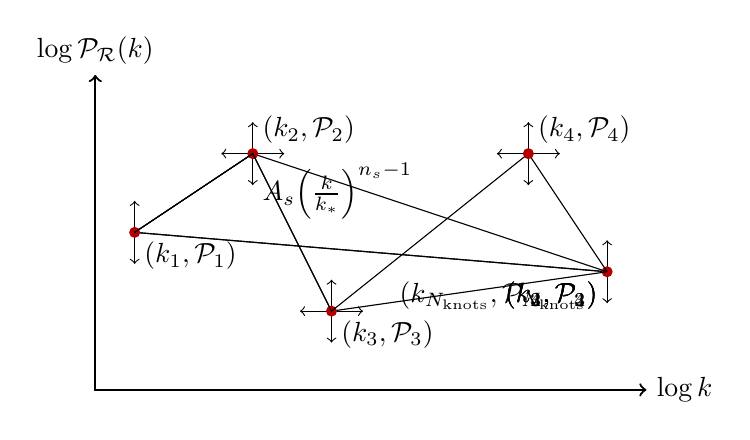
\begin{tikzpicture}
    % width of axes
      \def\xwidth{7}
      \def\ywidth{4}
    % min coordinate
      \def\xmn{0.5}
      \def\ymn{2}
    % start coordinate
      \def\xstart{2}
      \def\ystart{3}
    % middle coordinate
      \def\xmid{3}
      \def\ymid{1}
    % end coordinate
      \def\xend{5.5}
      \def\yend{3}
    % max coordinate
      \def\xmx{6.5}
      \def\ymx{1.5}

    % length of crosses
      \def\croslen{0.4}


    % Draw axes
      \draw [<->,thick] (0,\ywidth) node (yaxis) [above] {$\log\PR(k)$}
      |- (\xwidth,0) node (xaxis) [right] {$\log k$};
    % Draw limits
      %\draw [-,dashed] (\xmn,0) node[below] {$\log_{10}k_1$} -- (\xmn,\ywidth) ;
      %\draw [-,dashed] (\xmx,0) node[below] {$\log_{10}k_N$} -- (\xmx,\ywidth) ;

      \draw<1> (\xmn,\ymn) -- (\xmx,\ymx);
      \draw<1> (\xstart,\ystart) node[below right] {$A_s {\left(\frac{k}{k_*}\right)}^{n_s-1}$};

    % Draw the line joining start and end

      \coordinate (mn) at (\xmn,\ymn);
      \coordinate (start) at (\xstart,\ystart);
      \coordinate (mid) at (\xmid,\ymid);
      \coordinate (end) at (\xend,\yend);
      \coordinate (mx) at (\xmx,\ymx);
      \draw<2> (mn) -- (mx);
      \draw<2-> (mn) node[below right]    {$(k_1,\Pknotj{1})$};
      \draw<2> (mx) node[below left]     {$(k_{2},\Pknotj{{2}})$};
      \onslide<2->{\movablevert{mn}};
      \onslide<2->{\movablevert{mx}};

      \draw<3> (mn) -- (start) -- (mx);
      \onslide<3->{\movablecross{start}};
      \draw<3-> (start) node[above right] {$(k_2,\Pknotj{2})$};
      \draw<3> (mx) node[below left]     {$(k_{3},\Pknotj{{3}})$};
 
      \draw<4> (mn) -- (start) -- (mid) -- (mx);
      \onslide<4->{\movablecross{mid}};
      \draw<4-> (mid) node[below right] {$(k_3,\Pknotj{3})$};
      \draw<4> (mx) node[below left]     {$(k_{4},\Pknotj{{4}})$};

      \draw<5-> (mn) -- (start) -- (mid) -- (end) -- (mx);
      \onslide<5->{\movablecross{end}};
      \draw<5-> (end) node[above right] {$(k_4,\Pknotj{4})$};
      \draw<5-> (mx) node[below left]     {$(k_{\Nknots},\Pknotj{{\Nknots}})$};


      %\draw<2-> (\xmn,\ymn) coordinate (mn) -- (\xstart,\ystart) coordinate (start) -- (\xmid,\ymid) coordinate (mid) --  (\xend,\yend) coordinate(end) -- (\xmx,\ymx) coordinate(mx);

    % Draw the point labels
      %\draw<2-> (mn) node[below right]    {$(k_1,\Pknotj{1})$};
      %\draw<2-> (start) node[above right] {$(k_2,\Pknotj{2})$};
      %\draw<2-> (mid) node[below right]   {$(k_3,\Pknotj{3})$};
      %\draw<2-> (end) node[above right]   {$(k_4,\Pknotj{4})$};
      %\draw<2-> (mx) node[below left]     {$(k_{\Nknots},\Pknotj{{\Nknots}})$};

    % Draw a dashed line indicating the coordinate names
      %\draw[dashed] (yaxis |- start) node[left] {$y_{1}$}
      %-| (xaxis -| start) node[below] {$x_1$};
      %\draw[dashed] (yaxis |- mid) node[left] {$y_{2}$}
      %-| (xaxis -| mid) node[below] {$x_2$};
      %\draw[dashed] (yaxis |- end) node[left] {$y_{N}$}
      %-| (xaxis -| end) node[below] {$x_N$};
      %\draw  (xaxis -| start) node[below] {$\log_{10}k_2$};
      %\draw  (xaxis -| mid) node[below] {$\log_{10}k_3$};
      %\draw  (xaxis -| end) node[below] {$\log_{10}k_4$};

      % Draw the crosses
      %\onslide<2->{\movablevert{mn}
      %\movablecross{start}
      %\movablecross{mid}
      %\movablecross{end}
      %\movablevert{mx}
    %};

    % put some ellipses in between the start and end point

    \end{tikzpicture}

  }

\end{frame}


%\begin{frame}
%  \frametitle{Planck data}
%  \framesubtitle{Primordial power spectrum $\PR(k)$ reconstruction}
%  \begin{itemize}
%    \item<2-> Temperature data TT+lowP
%    \item<3-> Foreground $(14)$ \& cosmological $(4 +2*\Nknots-2)$  parameters
%    \item<4-> Marginalised plots of $\PR(k)$
%    \item<5->
%      \[ \prob(\PR|k,\Nknots) = \int \delta(\PR-f(k;\theta))\posterior(\theta)d\theta \]
%  \end{itemize}
%\end{frame}



\begin{frame}
  \frametitle<1>{0 internal knots}
  \frametitle<2>{1 internal knots}
  \frametitle<3>{2 internal knots}
  \frametitle<4>{3 internal knots}
  \frametitle<5>{4 internal knots}
  \frametitle<6>{5 internal knots}
  \frametitle<7>{6 internal knots}
  \frametitle<8>{7 internal knots}
  \frametitle<9>{8 internal knots}
  \frametitle<10>{Bayes Factors}
  \frametitle<11>{Marginalised plot}
  \framesubtitle{Primordial power spectrum $\PR(k)$ reconstruction}


  \begin{center}
    \includegraphics<1>[width=0.9\textwidth]{figures/0TT_fgivenx}
    \includegraphics<2>[width=0.9\textwidth]{figures/1TT_fgivenx}
    \includegraphics<3>[width=0.9\textwidth]{figures/2TT_fgivenx}
    \includegraphics<4>[width=0.9\textwidth]{figures/3TT_fgivenx}
    \includegraphics<5>[width=0.9\textwidth]{figures/4TT_fgivenx}
    \includegraphics<6>[width=0.9\textwidth]{figures/5TT_fgivenx}
    \includegraphics<7>[width=0.9\textwidth]{figures/6TT_fgivenx}
    \includegraphics<8>[width=0.9\textwidth]{figures/7TT_fgivenx}
    \includegraphics<9>[width=0.9\textwidth]{figures/8TT_fgivenx}
    \includegraphics<10>[width=0.9\textwidth]{figures/Bayes_TT.pdf}
    \includegraphics<11>[width=0.9\textwidth]{figures/combined_fgivenx.pdf}

  \end{center}
\end{frame}

\begin{frame}
    \frametitle{Dark energy equation of state reconstruction}
    \begin{itemize}
        \pause\item Same thing, but for Dark energy equation of state $w(z)$ (quintessence).
        \pause\item Data used is Planck 2015, BOSS DR 11, JLA supernovae and BOSS Ly$\alpha$ data
    \end{itemize}
\end{frame}
\begin{frame}
    \frametitle<1>{Flat, variable $w$}
    \frametitle<2>{Tilted}
    \frametitle<3>{1 internal node}
    \frametitle<4>{2 internal nodes}
    \frametitle<5>{3 internal nodes}
    \frametitle<6>{Marginalised plot - just extension models}
    \frametitle<7>{Marginalised plot - including LCDM}
    \framesubtitle{Dark energy equation of state reconstruction}

    \begin{center}
        \includegraphics<1>[width=0.9\textwidth]{figures/wCDM_1000Nlive_wgiivenz.pdf}
        \includegraphics<2>[width=0.9\textwidth]{figures/tCDM_100Nlive_wgiivenz.pdf}
        \includegraphics<3>[width=0.9\textwidth]{figures/1CDM_1000Nlive_wgiivenz.pdf}
        \includegraphics<4>[width=0.9\textwidth]{figures/2CDM_1000Nlive_wgiivenz.pdf}
        \includegraphics<5>[width=0.9\textwidth]{figures/3CDM_1000Nlive_wgiivenz.pdf}
        \includegraphics<6>[width=0.9\textwidth]{figures/extensionModels_1000Nlive_wgivenz.pdf}
        \includegraphics<7>[width=0.9\textwidth]{figures/allModels_1000Nlive_wgivenz.pdf}
    \end{center}
\end{frame}


\begin{frame}
    \frametitle{Useful links}
    \begin{description}
        \item[My email:] wh260@cam.ac.uk
        \item[My room:] Room 104, Tuesday-Thursday this week
        \item[PolyChord:] ccpforge.cse.rl.ac.uk/gf/project/polychord
        \item[MultiNest:] ccpforge.cse.rl.ac.uk/gf/project/multinest
        \item[Stan:] mc-stan.org/
        \item[emcee:] dan.iel.fm/emcee/current/
    \end{description}
\end{frame}

\end{document}
